\documentclass[11pt, a4paper]{article}
\usepackage[margin=1in]{geometry}

\usepackage{lmodern}
\fontfamily{lmdh}\selectfont

\usepackage{graphicx}
\graphicspath{{images}}

\usepackage{titlesec}
\titleformat*{\section}{\large\bfseries}

\usepackage{caption}
\captionsetup[figure]{font={small, bf}}

\usepackage{subcaption}

\usepackage[style=authoryear-ibid,backend=biber]{biblatex}
\renewcommand*{\nameyeardelim}{\addcomma\space}
\addbibresource{ag_bib.bib}

\usepackage{verbatim}

\title{\Large\bfseries Classification and Pricing of Farmed Abalone}
\author{\large Amanjit Gill}
\date{\small \today}

\begin{document}
    
    \maketitle

    \section*{Introduction}    
      
    An enquiry has been made as to the potential use of software to help abalone farmers to quickly assess whether an abalone should be harvested or left in the water. The aim is to use non-intrusive measurements - length, diameter and height - to predict an abalone's sex and infancy status, as well as its weight (and thus market value), allowing farmers to return rejected abalone to the water without having harmed them.

    \section{Exploratory Analysis}

    Data on more than 4000 harvested abalone have been supplied. The dataset includes the following columns (variables):

    \begin{itemize}
        \item Sex
        \item Length, diameter and height
        \item Whole, shucked, viscera and shell weights
        \item Number of rings on the shell (an indicator of age)
    \end{itemize}

    The data have been checked for missing or impossible values. No entries are missing, but two abalone have a recorded height of 0, a physical impossibility. These two rows have been removed.

    The data analysis techniques to be used depend on the supplied data meeting certain conditions \parencite{assumptions}:

    \begin{itemize}
        \item \textbf{Normality.} When the probability of each value occurring is graphed against the value itself, the curve (known as a density plot) should form the classical bell shape expected of ``normal'' data.
        \item \textbf{Linearity.} The relationship between each pair of variables should be linear.
        \item \textbf{Homoscedasticity.} The variation (spread) in one variable should remain the same, regardless of the value of another variable. 
    \end{itemize}

    \subsection{Normality}

    The density plots for all the numerical variables are shown in Figure \ref{density}.

    \begin{figure}[hbt!]
        \centering
        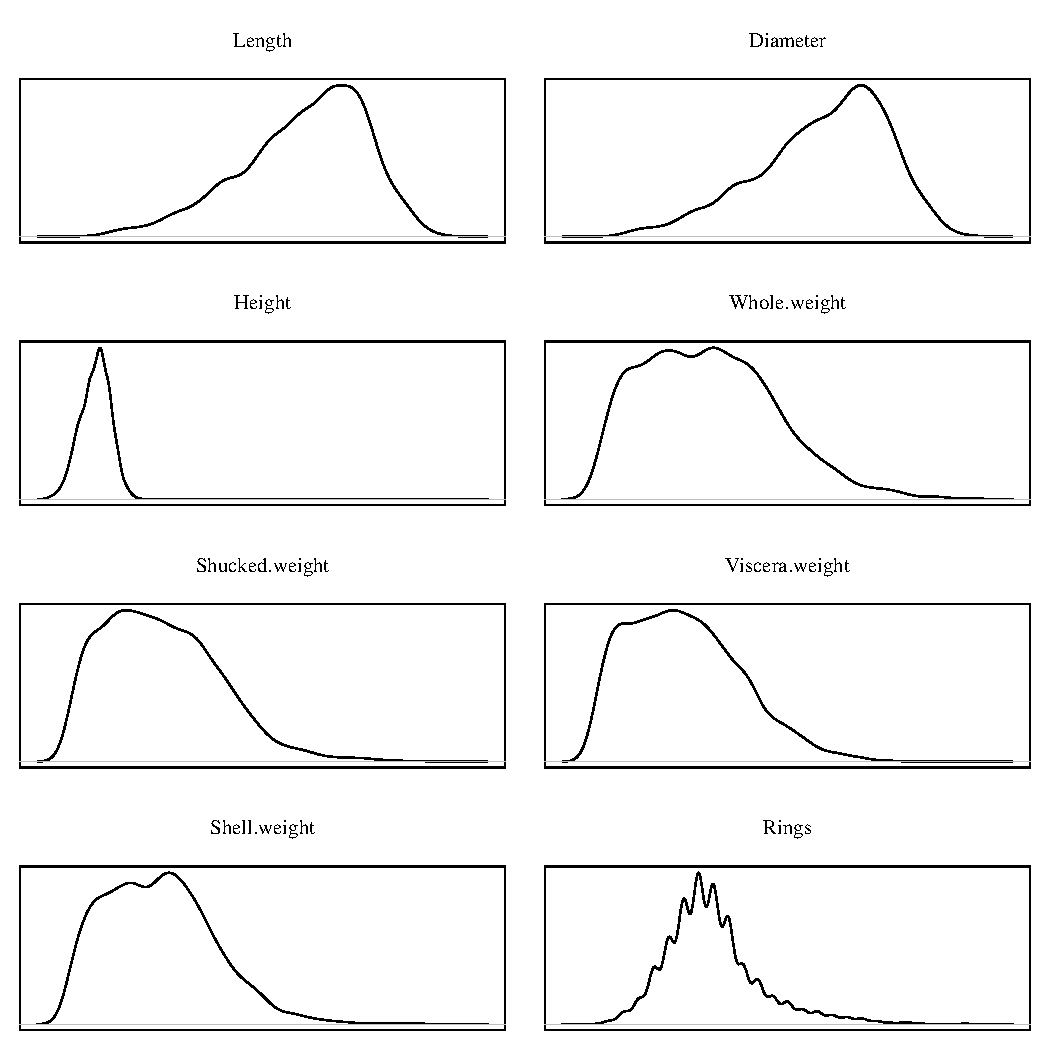
\includegraphics[width=\textwidth]{1.4.pdf}
        \caption{Density Plots}
        \label{density}
    \end{figure}

    All of the variables are skewed; that is, the bell curve is stretched either left or right. This can be repaired, to some extent, by transforming the data i.e. altering the values to force them into a more symmetrical shape \parencite{transformations}.

    \subsection{Linearity and Homoscedasticity}

    These two requirements can be checked by plotting pairs of the variables against one another, as shown in Figure \ref{pairs}. The following observations can be made:

    \begin{itemize}
        \item The relationships between all the weight variables, and the length and diameter, are non-linear.
        \item The slightly oval shape of the plots pairing the four weights suggests that these variables are normally distributed \parencite{assumptions}. Examining Figure \ref{density} confirms that the four weight variables are the most ``normal'', with low kurtosis (pointiness) but some skew to the right.
    \end{itemize}

    \begin{figure}[hbt!]
        \centering
        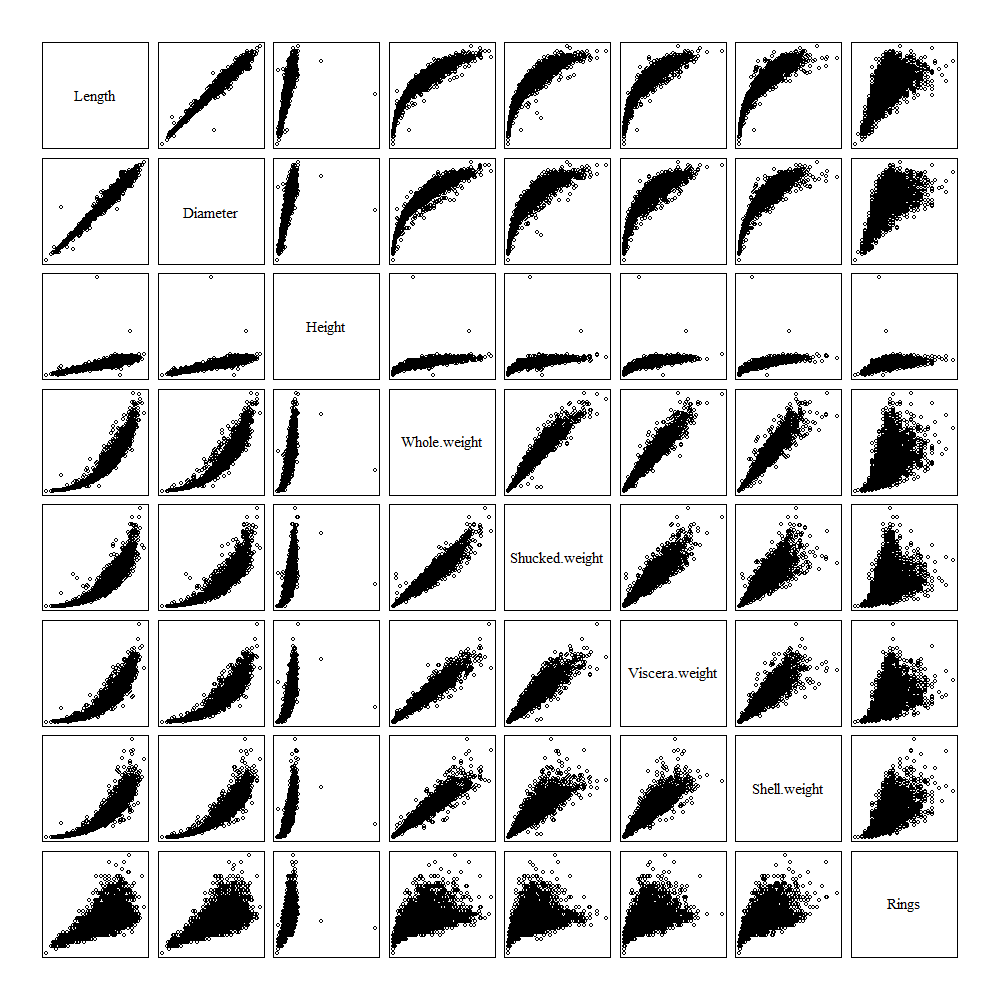
\includegraphics[width=\textwidth]{1.3.png}
        \caption{Scatter Plots of Variable Pairs}
        \label{pairs}
    \end{figure}

    \subsection{Data Correction}

    Transformations have the benefit of pulling outliers (extreme values) in towards the centre, so that they are no longer considered extreme. Then, any remaining outliers may be removed from the dataset. Transformations also help to improve the linearity of the relationships between the variables \parencite{transformations}.

    Table \ref{outliers} shows that most outliers have been successfully addressed by transformations, leaving only a small number to be removed from the dataset (with the exception of height). Figure \ref{density.t} illustrates a substantial improvement in every variable, after applying a transformation and removing the remaining outliers. 
    
    \begin{table}[ht]
        \centering
        \begin{tabular}{|l|c|c|}
            \hline
            Variable&Initial Outliers&Remaining Outliers \\
            \hline
            Length & 49 & 8 \\
            Diameter & 59 & 9 \\
            Height & 27 & 156 \\
            Whole weight & 30 & 1 \\
            Shucked weight & 48 & 3 \\
            Viscera weight & 26 & 2 \\
            Shell weight & 35 & 8 \\
            Rings & 278 & 268 \\
            \hline
        \end{tabular}
        \caption{Outliers Before and After Transformations}
        \label{outliers}
    \end{table}

    \begin{figure}[hbt!]
        \centering
        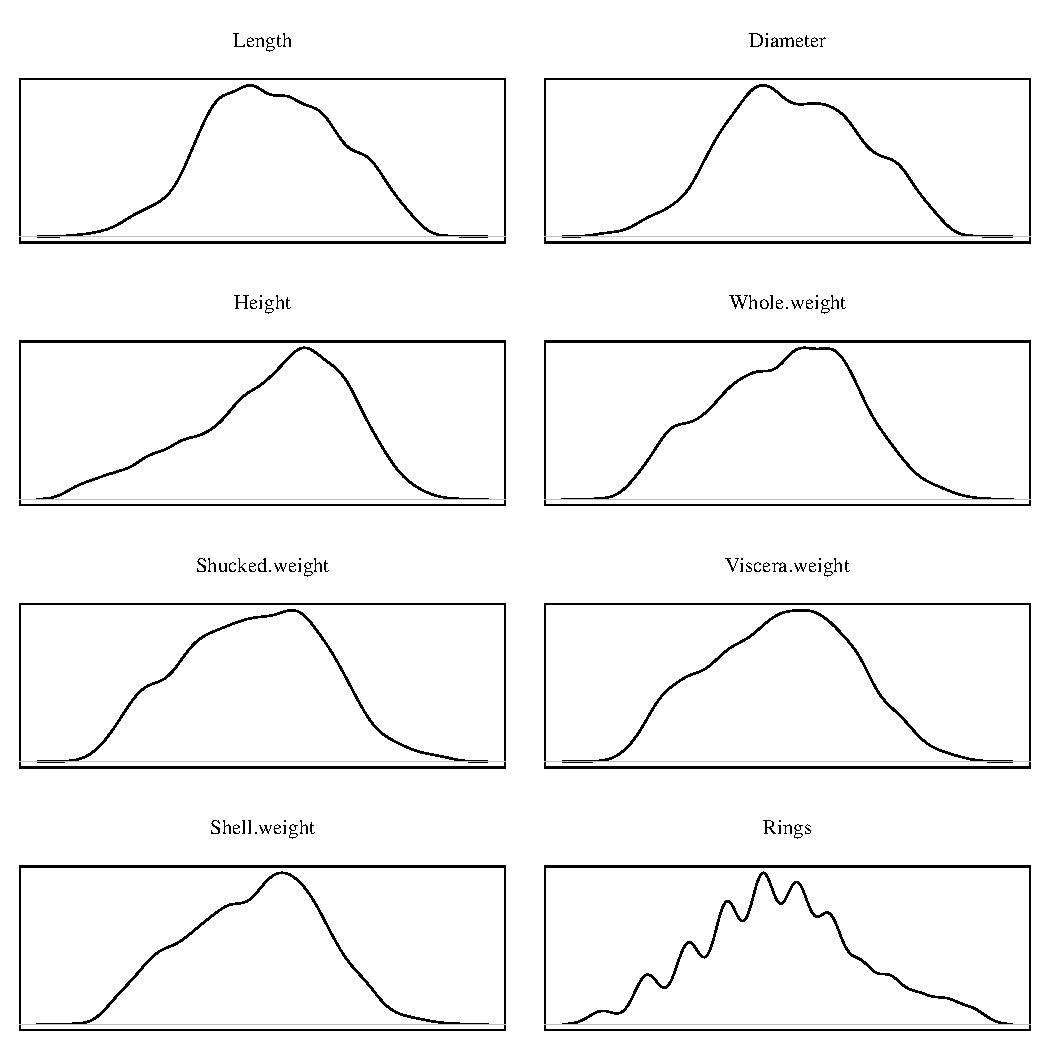
\includegraphics[width=\textwidth]{1.7.pdf}
        \caption{Density Plots After Transformations and Removal of Outliers}
        \label{density.t}
    \end{figure}

    Having confirmed, through analysis of skewness and kurtosis \parencite{assumptions}, that the variables are now much closer to ``normal'', data modelling to predict sex and infancy status can now proceed.

    \section{Predicting Sex and Infancy}

    The supplied data have been fed into two machine learning algorithms in order to develop a ``classifier'' that labels an abalone an infant, female or male, based on non-intrusive measurements (length, diameter and height). 

    The first algorithm involves \textbf{discriminant analysis} \parencite{da}; the second involves a \textbf{support vector machine} (SVM) \parencite{svm}.

    \subsection{Three-Way Classifier}

    Table \ref{three-way} reports the accuracy for each of the attempted algorithms.

    \begin{table}[ht]
        \centering
        \begin{tabular}{|l|c|}
            \hline
            Model & Accuracy \% \\
            \hline
            quadratic discriminant analysis (QDA) & 0.5050 \\
            linear discriminant analysis (LDA) & 0.5153 \\
            linear SVM & 0.5147 \\
            radial SVM & 0.5168 \\
            \hline
        \end{tabular}
        \caption{Accuracy of Three-Way Classifiers}
        \label{three-way}
    \end{table}

    The overall accuracy for all models is poor, but is slightly better for SVM. Table \ref{svm-acc} shows the accuracy of the two SVM models by sex.

    \begin{table}[ht]
        \centering
        \begin{tabular}{|l|c|c|}
            \hline
            Class & Accuracy (Linear) \% & Accuracy (Radial) \% \\
            \hline
            Infant & 0.7206 & 0.7121 \\
            Female & 0 & 0.0025 \\
            Male & 0.7820 & 0.7926 \\
            \hline
        \end{tabular}
        \caption{Accuracy of SVM Classifiers by Sex and Infancy}
        \label{svm-acc}
    \end{table}

    Nearly all of the female abalone are labelled incorrectly by these models. By contrast, their accuracy is acceptable (above 70\%) for infants, and approaching good (nearly 80\%) for males. In order to understand this phenomenon, the three input variables can be grouped by sex and infancy status, as shown in Figure \ref{boxplots}.

    \begin{figure}[hbt!]
        \centering
        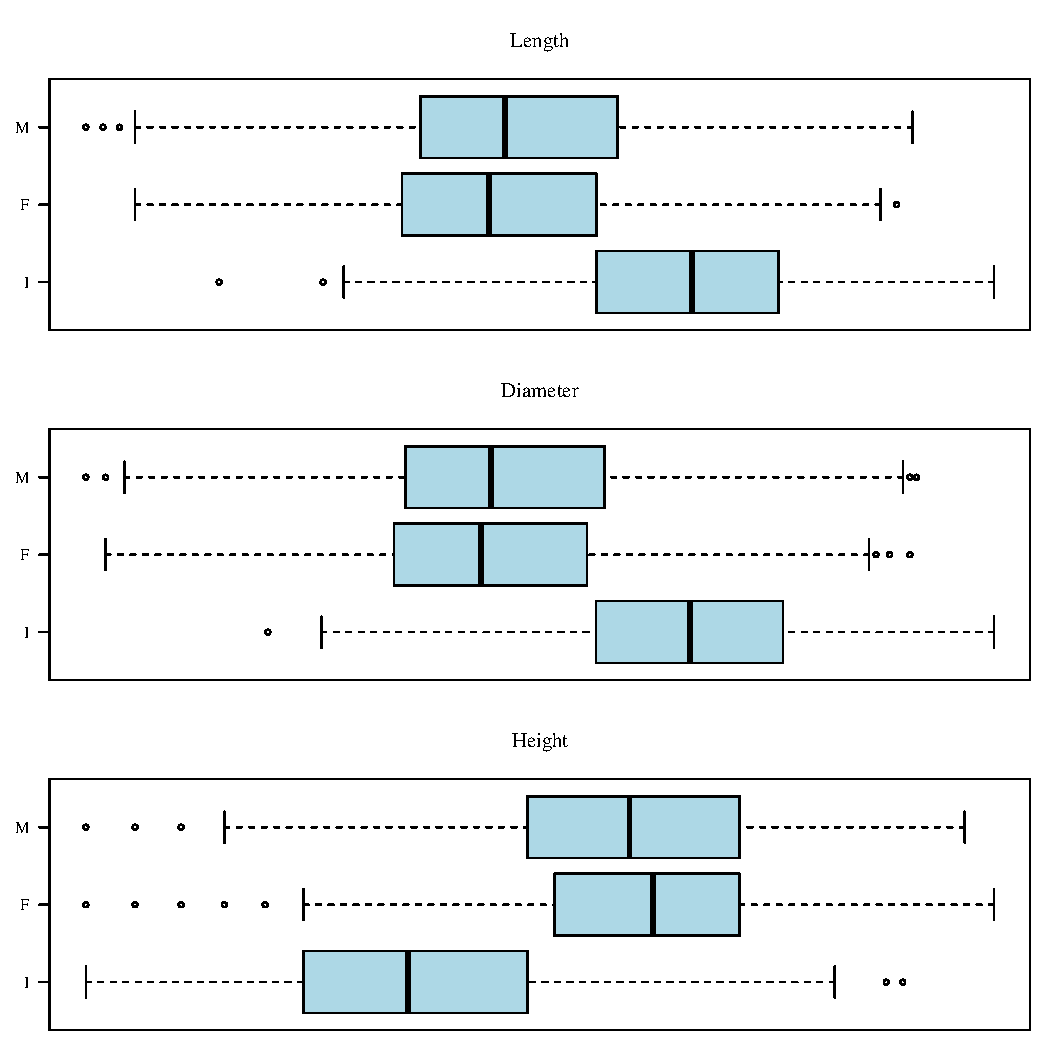
\includegraphics[width=\textwidth]{2.4.pdf}
        \caption{Input Variables by Sex Class}
        \label{boxplots}
    \end{figure}

    The boxplots show that the values of length, diameter and height for males and females overlap, while the values for infants are substantially separated from the sexes. This explains why the models are unable to differentiate between males and females.

    Because of this, \textbf{none} of the models is suitable as a three-way classifier.

    \subsection{Binary Classifiers}

    Having failed to specify a three-way classifier, binary classifiers have been attempted, to differentiate between:

    \begin{itemize}
        \item Infants and non-infants, to avoid harvesting infant abalone
        \item Females and non-females, to selectively harvest females for increased profits \parencite{atlantic}
        \item Males and non-males, to selectively harvest males to preserve female populations
    \end{itemize}

    A performance summary for the best models in these scenarios is given in Table \ref{binary}. While it appears that all three models perform reasonably well, closer inspection indicates otherwise. From the \textbf{confusion matrix} shown in Table \ref{cms}:

    \begin{itemize}
        \item \textbf{I vs Not I}: Good at identifying non-infants, but poor at positively identifying infants.
        \item \textbf{F vs Not F}: Classifies nearly all abalone as non-female, regardless of true sex.
        \item \textbf{M vs Not M}: Classifies nearly all abalone as non-male, regardless of true sex.
    \end{itemize} 
 
    \begin{table}[ht]
        \centering
        \begin{tabular}{|l|l|c|}
            \hline
            Classifier  & Best Model    & Accuracy \% \\
            \hline
            I vs Not I  & SVM radial    & 0.7950 \\
            F vs Not F  & SVM radial    & 0.6926 \\
            M vs Not M  & SVM radial    & 0.6824 \\
            \hline
        \end{tabular}
        \caption{Accuracy of Binary Classifiers}
        \label{binary}
    \end{table}

    \begin{table}
        \centering
        \begin{tabular}{|l|c|c|}
            \hline
                            & Predicted & Predicted Not \\
            \hline
            Actual I        & 675       & 506 \\
            Actual Not I    & 273       & 2346 \\
            \hline
            Actual F        & 84        & 1122 \\
            Actual Not F    & 46        & 2548 \\
            \hline
            Actual M        & 1         & 1412 \\
            Actual Not M    & 0         & 2387 \\
            \hline           
        \end{tabular}
        \caption{Confusion Matrix for Binary Classifiers}
        \label{cms}
    \end{table}

    Therefore, it is recommended that a binary classifier for infants and non-infants \textbf{only} be used to identify non-infants, not for positively identifying infants. In addition, it is recommended that a binary classifier \textbf{not} be used at all for females and non-females, and males and non-males.

    Unfortunately, this means that the objective to use non-intrusive measurements to predict the sex of abalone cannot be met, because males and females are not differentiable by their physical proportions \parencite{nsw}.

    \section{Estimating Value}

    By returning smaller (and likely younger) abalone to the water and allowing them to mature and reproduce, farmers can ensure sustainability of abalone populations, while maximising profits by selectively harvesting larger (presumably older) abalone with more meat.

    To this end, a function has been developed by which a farmer can quickly predict the shucked and viscera weights of an abalone, based only on its measurements, and thus estimate the market value. A \textbf{multiple linear regression} (MLR) model has been fed summaries of the transformed data for length, diameter, height and the two weights of interest. The resulting prediction equations are:

    $$ Shucked\_weight\_t = 15.768 - 1.14*Length\_t - 0.432*Diameter\_t + 1.164*Height\_t $$
    $$ Viscera\_weight\_t = 7.145 - 0.698*Length\_t - 0.256*Diameter\_t + 1.691*Height\_t $$

    Figure \ref{mlr} shows that there is very good agreement between actual abalone weights and the weights predicted by these equations. An alternative model involving \textbf{principal component analysis} \parencite{pca} also yields good results, but the above MLR equations are slightly superior.

    \begin{figure}[hbt!]
        \centering
        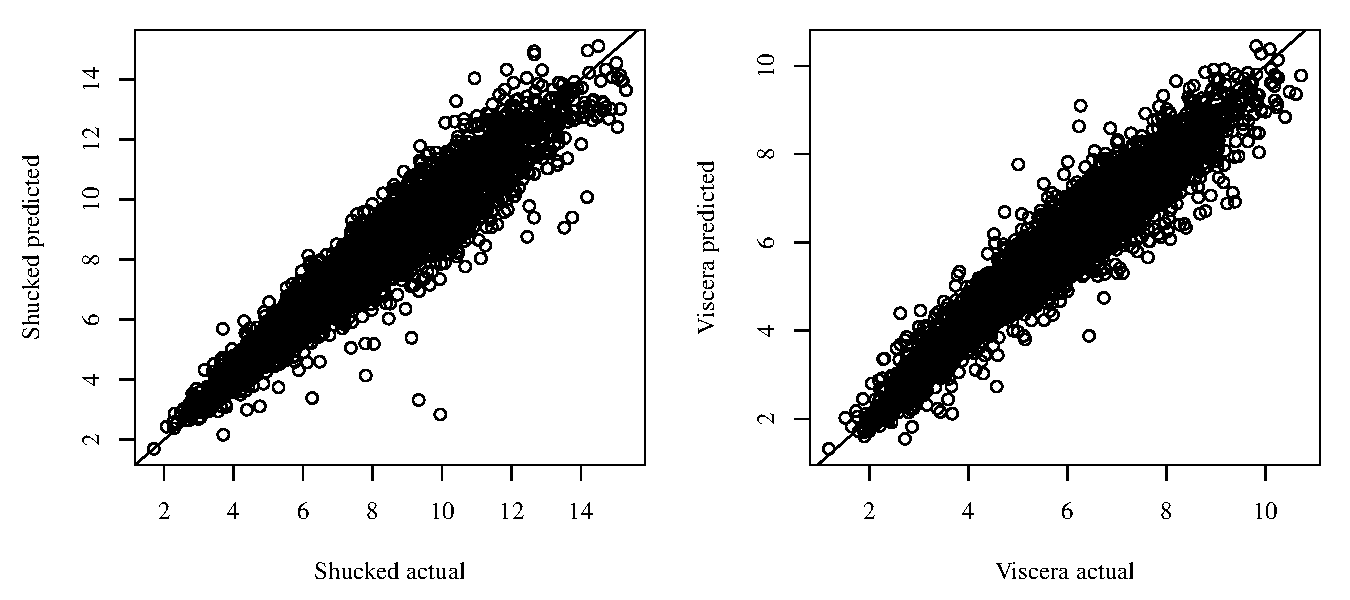
\includegraphics[width=\textwidth]{3.2.pdf}
        \caption{Predicted vs Actual Weights}
        \label{mlr}
    \end{figure}

    The weights in the supplied data were originally transformed by taking the square root, so the opposite operation (square) converts them to their original units:

    $$ Shucked\_weight = Shucked\_weight\_t ^ 2 $$
    $$ Viscera\_weight = Viscera\_weight\_t ^ 2 $$

    The market price for one abalone is thus estimated:

    $$ Est\_Price = Shucked\_weight * Price\_per\_gram_{sh} + Viscera\_weight * Price\_per\_gram_{vi} $$

    This price estimate is accompanied by a prediction interval \parencite{pi}, the bounds of which are determined by the end user (e.g. for a 90\% prediction interval, alpha is set to 0.1). The final function thus has inputs and outputs as shown in Table \ref{function}.

    \begin{table}[ht]
        \centering
        \begin{tabular}{|c|c|}
            \hline
            Inputs & Outputs \\
            \hline
            length (mm) & estimated price (\$) \\
            diameter (mm) & lower bound (\$) \\
            height (mm) & upper bound (\$) \\
            price/gram, shucked (\$) & \\
            price/gram, viscera (\$) & \\
            alpha (default 0.05) & \\
            \hline
        \end{tabular}
        \caption{Inputs and Outputs of Price Estimator}
        \label{function}
    \end{table}

    \section*{Conclusion}

    The aims of this study have partially been met. Using dimensional measurements alone, it is currently not possible to balance competing interests in sustainability and profitability by selectively harvesting for sex. However, there is scope, through the infant vs non-infant classifier in conjunction with the price estimation function, to improve farming practices by selectively harvesting larger and more mature abalone.

    \printbibliography

    \nocite{*}

\end{document}

